% MarsPulse Final Report — English Version
% Compiled with: xelatex marspulse_EN.tex
\documentclass[11pt,a4paper]{article}

% ─── Packages ────────────────────────────────────────────────────────
\usepackage{fontspec}
\usepackage{geometry}
\geometry{margin=2.5cm}
\usepackage{graphicx}
\usepackage{amsmath,amssymb}
\usepackage{booktabs}
\usepackage{hyperref}
\usepackage{caption}
\usepackage{subcaption}
\usepackage{enumitem}
\usepackage{fancyhdr}
\usepackage{titlesec}
\usepackage{xcolor}
\usepackage{float}
\usepackage{multirow}
\usepackage{makecell}
\hypersetup{
  colorlinks=true,
  linkcolor=blue!60!black,
  citecolor=blue!40!black,
  urlcolor=blue!60!black,
}

% ─── Style ──────────────────────────────────────────────────────────
\titleformat{\section}{\Large\bfseries}{\thesection}{1em}{}
\titleformat{\subsection}{\large\bfseries}{\thesubsection}{1em}{}
\pagestyle{fancy}
\fancyhf{}
\fancyhead[L]{\small MarsPulse: MARL-Based Mars Lava Tube Base Resource Management}
\fancyhead[R]{\small\thepage}
\renewcommand{\headrulewidth}{0.4pt}

\graphicspath{{../output/}}

% ─── Title ──────────────────────────────────────────────────────────
\title{
  \vspace{2cm}
  {\huge\textbf{MarsPulse}}\\[8pt]
  {\Large MARL-Based Resource Management for a Mars Subsurface Lava Tube Base}\\[20pt]
  \large Final Technical Report\\[5pt]
  \normalsize Steps 1--5: Physical Modeling Through MARL Validation
}
\author{}
\date{June 2, 2026}

\begin{document}

\maketitle
\thispagestyle{empty}

\vspace{3cm}
\begin{center}
  \large
  \textbf{Research Domain:} Deep Space Exploration / Aerospace + AI \\
  \textbf{Keywords:} Mars lava tube base, ISRU, Multi-Agent RL, MAPPO,\\
  survival boundary simulation, autonomous decision-making
\end{center}

\newpage

% ─── Abstract ────────────────────────────────────────────────────────
\begin{center}
  \Large\textbf{Abstract}
\end{center}
\vspace{8pt}

Long-duration Mars habitation must contend with severe environmental conditions and communication delays that preclude real-time ground control. This project studies the survival stability of a Mars subsurface lava tube base under global dust storms---events that can cut surface solar power by over 80\% for extended periods. The scenario models a 300-sol Mars year with two dust storms (sol~60--120 at optical depth $\tau=2.5$, and sol~200--235 at $\tau=2.2$), a 3,000~kWh battery bank, a 150~kW solar array, and a 10~kW RTG.

We formulate the base's power, thermal, and oxygen management as a cooperative multi-agent problem and train three MAPPO agents with a centralized critic over 300,000 environment steps. In a 100-episode Monte Carlo evaluation, the MARL policy extends mean survival from 123.7~sols (static rule-based baseline, same seed set) to 167.2~sols, an improvement of 35.2\%. 37\% of MARL episodes achieve full 300-sol survival versus 8\% for the static baseline. The fatality rate drops from 92\% to 63\%.

Ablation experiments find that single-agent PPO and independent multi-agent PPO both collapse to roughly 2.5~sols on this task---the centralized critic provides a 127-sol improvement, suggesting that inter-agent coordination is not merely helpful but necessary at this horizon. Parameter sensitivity analysis further shows that static agent survival is almost entirely insensitive to battery capacity (1,000--5,000~kWh yields $\sim$118~sols uniformly), indicating that the bottleneck lies in decision architecture rather than hardware sizing.

\vspace{10pt}
\noindent\textbf{Keywords:} deep space exploration, aerospace + AI, lava tube base, ISRU, multi-agent reinforcement learning, MAPPO, survival boundary simulation.

\newpage

% ─── TOC ─────────────────────────────────────────────────────────────
\tableofcontents
\newpage

%======================================================================
\section{Introduction \& Research Background}
%======================================================================

\subsection{Mars Lava Tube Habitats}

The surface of Mars is a difficult place to live. Galactic cosmic ray and solar particle radiation reaches roughly 0.67~mSv/day~\cite{mars_radiation}, diurnal temperatures swing from $-100^\circ$C to 20$^\circ$C, and the thin atmosphere offers negligible protection against micrometeorites. Lava tubes---natural subsurface caverns formed by ancient basaltic flows~\cite{mars_lava_tube}---have attracted interest as habitat sites for three reasons:

\begin{enumerate}[label=(\roman*)]
  \item \textbf{Radiation shielding:} Several meters of basalt overburden block the majority of high-energy particles.
  \item \textbf{Thermal stability:} Temperatures at 10--20~m depth hold near $-20^\circ$C year-round, removing the diurnal extremes that dominate surface thermal design.
  \item \textbf{Structural integrity:} Pre-existing rock ceilings eliminate the need to launch and assemble heavy radiation shielding.
\end{enumerate}

\subsection{The Decision-Making Problem During Dust Storms}

Regional and global dust storms occur regularly on Mars~\cite{mars_dust}. During a major storm, atmospheric optical depth can exceed $\tau = 2.5$, reducing surface solar irradiance to below 10\% of clear-sky levels for 60~sols or longer. The same atmospheric dust that attenuates sunlight also degrades direct-to-Earth radio links, and orbital geometry may place Earth below the horizon for extended periods. The result is a ``blackout island'': the crew must manage resources autonomously, without ground intervention, while energy input collapses.

Conventional spacecraft resource management follows \textbf{static rule-based protocols}---pre-programmed contingency tables with fixed priority chains (life support first, then thermal control, then payloads). These protocols are straightforward to validate and have extensive flight heritage, but they share known limitations:

\begin{itemize}
  \item \textbf{Rigidity under compound failures:} Fixed priority lists cannot re-order themselves when two subsystems degrade simultaneously.
  \item \textbf{Reactive rather than anticipatory:} Rules trigger when a measurement crosses a threshold; they do not project trajectories forward.
  \item \textbf{Subsystem-local perspective:} Each subsystem controller optimizes its own margins without visibility into cross-system effects, such as equipment waste heat offsetting heating demand.
\end{itemize}

We examine whether a \textbf{Multi-Agent Reinforcement Learning (MARL)} approach~\cite{marl_survey} can improve on these limitations by learning resource-allocation strategies that adapt to the specific storm conditions and failure states encountered.

%======================================================================
\section{Physical Models \& Parameter Justification}
%======================================================================

This section defines the mathematical description of the base and explains where each parameter value comes from.

\subsection{Survival Stability Index}

We define a single scalar $S(t) \in [0,1]$ that collapses three resource dimensions into a health metric:

\begin{equation}\label{eq:S}
  S(t) = w_E \cdot E(t) + w_O \cdot O(t) + w_T \cdot T(t)
\end{equation}

$E(t) = E_{\text{stored}} / E_{\text{capacity}}$ is the battery state-of-charge fraction. $O(t) = M_{O_2} / M_{O_2}^{\text{max}}$ is the oxygen storage fraction. $T(t) = 1 - |T_h - T_{\text{target}}| / (T_{\text{max}} - T_{\text{min}})$ is a thermal comfort score that equals 1 at the 20$^\circ$C setpoint and falls to 0 at the survivable bounds of 5$^\circ$C and 35$^\circ$C.

The weights are $(w_E, w_O, w_T) = (0.40, 0.35, 0.25)$. Electricity receives the largest weight because both oxygen generation (electrolysis) and active thermal control depend on it. Oxygen ranks second as the most time-critical consumable directly tied to crew survival; thermal comfort ranks third because the lava tube's thermal mass provides passive buffering. A state with $S(t) < 0.15$ is classified as critical risk; $S(t) < 0.05$ is considered fatal and the episode terminates.

\subsection{Solar Power Input}

Surface solar power during a dust storm follows the Beer-Lambert extinction law:

\begin{equation}\label{eq:solar}
  P_{\text{in}}(t) = P_{\text{max}} \cdot \eta \cdot e^{-\tau(t)} \cdot \cos(\theta) + P_{\text{rtg}}
\end{equation}

\textbf{Parameter values and their origins:}
\begin{itemize}
  \item $P_{\text{max}} = 150$~kW: This represents roughly 750~m$^2$ of photovoltaic area. The solar constant at Mars' orbital distance is about 590~W/m$^2$; after passage through a clear atmosphere and accounting for $\sim$20\% cell efficiency, practical surface output is roughly 100~W/m$^2$. 750~m$^2$ is plausible for a medium-scale base and could be deployed as lightweight roll-out arrays.
  \item $\eta = 0.85$: Accounts for dust accumulation between cleaning cycles, array aging, and DC/AC conversion losses.
  \item $\tau(t)$: Optical depth varies with dust loading. Under clear sky $\tau = 0.15$, giving $e^{-0.15} \approx 0.86$ transmission. During the major storm $\tau = 2.5$, giving $e^{-2.5} \approx 0.082$ transmission. The storm envelope follows a $\sin^{0.8}$ profile to approximate realistic onset and decay.
  \item $\theta$: Solar incidence angle. We use $\bar{\theta} = 0$ ($\cos\theta = 1.0$), corresponding to an equatorial site with Sun-tracking arrays at equinox. This is conservative in the sense that it overestimates available power at other latitudes and seasons; actual bases at higher latitudes would see lower input.
  \item $P_{\text{rtg}} = 10.0$~kW: Roughly equivalent to four Multi-Mission RTG units of the type flown on Perseverance ($\sim$2.7~kW each at beginning of life)~\cite{kilopower}. RTG output is independent of atmospheric conditions and provides the irreducible power floor.
\end{itemize}

At clear sky ($\tau = 0.15$): $P_{\text{in}} = 150 \times 0.85 \times 0.861 \times 1.0 + 10.0 \approx 109.8 + 10.0 \approx 119.8$~kW. At storm peak ($\tau = 2.5$): $P_{\text{in}} = 150 \times 0.85 \times 0.082 \times 1.0 + 10.0 \approx 10.5 + 10.0 \approx 20.5$~kW, an 83\% reduction from clear-sky conditions.

\subsection{Thermal Dynamics}

The habitat is modeled as a single lumped thermal mass exchanging heat with the surrounding rock:

\begin{equation}\label{eq:thermal}
  C_h \frac{dT_h}{dt} = Q_{\text{heater}} + Q_{\text{waste}} - k_h (T_h - T_{\text{rock}})
\end{equation}

\textbf{Parameter values and their origins:}
\begin{itemize}
  \item $C_h = 50,\!000$~kJ/$^\circ$C: This is the effective thermal mass of a $\sim$500~m$^3$ habitat. Dry air contributes roughly 1.2~kJ/m$^3\!\cdot\!$K; the dominant contribution is from structural materials, regolith shielding, equipment, and furnishings. The value is consistent with published Mars habitat thermal models~\cite{mars_thermal}.
  \item $T_{\text{rock}} = -20^\circ$C: Measured and modeled subsurface temperatures at 10--20~m depth in Martian regolith, where diurnal and seasonal variations are damped to near-constant values.
  \item $k_h = 0.18$~kW/$^\circ$C: Effective conductance through insulated habitat walls, corresponding to a U-value of $\sim$0.36~W/m$^2\!\cdot\!$K over $\sim$500~m$^2$ of surface area. Achievable with multi-layer aerogel insulation.
  \item $Q_{\text{waste}}$: 70\% of non-heating electrical load is assumed to dissipate as heat within the habitat, contributing passive warming.
  \item Heater capacity: 15~kW maximum, roughly three commercial-scale heat pump units.
  \item Survivability bounds: [$5^\circ$C, $35^\circ$C], following NASA crew habitat standards.
\end{itemize}

\subsection{Oxygen Mass Balance}

\begin{equation}\label{eq:o2}
  \frac{dM_{O_2}}{dt} = \eta_{\text{elec}} \cdot P_{\text{elec}} - n_{\text{crew}} \cdot \dot{m}_{\text{cons}}
\end{equation}

\begin{itemize}
  \item $\eta_{\text{elec}} = 0.15$~kg~O$_2$/kWh: Water electrolysis has a theoretical maximum of $\sim$0.25~kg/kWh; practical solid-oxide cells operating on Mars atmospheric CO$_2$ (similar to MOXIE-type ISRU) achieve roughly 60\% efficiency~\cite{mars_isru}.
  \item $n_{\text{crew}} = 6$: Representative crew for an initial permanent outpost.
  \item $\dot{m}_{\text{cons}} = 0.84$~kg/sol/person: NASA BVAD metabolic oxygen consumption standard, including a 20\% safety margin above the nominal resting rate~\cite{nasa_ls}.
  \item $M_{O_2}^{\text{max}} = 500$~kg: Provides roughly 99~sols of breathable oxygen for 6 crew with no regeneration, sufficient to ride out the longest plausible dust storm.
\end{itemize}

\subsection{Battery Energy Balance}

\begin{equation}\label{eq:battery}
  \frac{dE}{dt} = P_{\text{in}}(t) - P_{\text{load}}(t)
\end{equation}

$P_{\text{load}} = a_1 + a_2 + a_3 + P_{\text{misc}}$ sums the three agent-controlled loads plus fixed loads (lighting 4~kW, communications 3~kW). The battery capacity of 3,000~kWh supports roughly 10--12~sols of full operation without solar input. Charge/discharge rates are capped at $\pm 80$~kW. This capacity is roughly equivalent to 60 Tesla Model S battery packs or a dedicated vanadium redox flow battery installation.

%======================================================================
\section{MARL Architecture}
%======================================================================

\subsection{Agent Decomposition}

Three agents share control of the base, each with a scalar continuous action:

\begin{enumerate}[label=\textbf{Agent \arabic*:}]
  \item \textbf{Power Manager} --- allocates $a_1 \in [0, 30]$~kW to life support systems. Observes battery fraction, O$_2$ fraction, storm status, optical depth, and active failure flags.
  \item \textbf{Thermal Controller} --- allocates $a_2 \in [0, 20]$~kW to habitat heating. Observes temperature deviation, battery fraction, storm status, and failure flags.
  \item \textbf{Science Manager} --- allocates $a_3 \in [0, 25]$~kW to experiment payloads. Observes battery fraction, storm status, O$_2$ fraction, and failure flags.
\end{enumerate}

All agents receive the same cooperative reward, structured as a combination of survival time credit, S(t)-based health bonuses, and penalties for illegal (out-of-bounds) actions and fatal termination.

\subsection{MAPPO with Action Bounds}

We use Multi-Agent PPO (MAPPO)~\cite{mappo} with a centralized critic and decentralized actors. Each agent $i$ maintains a Gaussian policy $\pi_{\theta_i}(a_i | o_i)$. The raw network output $\mu_{\text{raw}}$ is passed through a $\tanh$ nonlinearity and linearly mapped to the valid range:

\begin{equation}\label{eq:tanh}
  \mu = \tanh(\mu_{\text{raw}}) \cdot \frac{a_{\text{high}} - a_{\text{low}}}{2} + \frac{a_{\text{high}} + a_{\text{low}}}{2}
\end{equation}

The log-standard-deviation is clipped to $[-4, 2]$ to prevent variance collapse. Sampled actions are additionally hard-clamped to $[a_{\text{low}}, a_{\text{high}}]$. Without these bounds, agents quickly discover that outputting negative power values (i.e., violating energy conservation) yields artificially high rewards. The bounded parameterization removes this non-physical pathway.

The central critic $V_\phi(s, \mathbf{a})$ receives the concatenated global state $s = [o_1, o_2, o_3]$ and the joint action $\mathbf{a} = [a_1, a_2, a_3]$. This allows the value function to represent cross-agent effects---for example, waste heat from life support equipment offsetting the thermal agent's heating burden, or the power agent and science agent competing for the same battery capacity.

The PPO clipped objective for each agent:

\begin{equation}\label{eq:ppo}
  \mathcal{L}_i(\theta_i) = \mathbb{E}_t\left[\min\left(r_t(\theta_i)\hat{A}_t,\; \text{clip}(r_t(\theta_i), 1-\epsilon, 1+\epsilon)\hat{A}_t\right)\right]
\end{equation}

where $r_t(\theta_i) = \pi_{\theta_i}(a_i|o_i) / \pi_{\theta_i^{\text{old}}}(a_i|o_i)$ and $\hat{A}_t$ is computed via Generalized Advantage Estimation~\cite{gae} with $\gamma = 0.995$ and $\lambda = 0.95$.

\subsection{Training Configuration}

\begin{table}[H]
  \centering
  \caption{Training hyperparameters}
  \label{tab:hparams}
  \begin{tabular}{@{}ll@{}}
    \toprule
    \textbf{Parameter} & \textbf{Value} \\
    \midrule
    Actor learning rate & $3 \times 10^{-4}$ (cosine annealing) \\
    Critic learning rate & $8 \times 10^{-4}$ (cosine annealing) \\
    Discount factor $\gamma$ & 0.995 \\
    GAE parameter $\lambda$ & 0.95 \\
    PPO clip ratio $\epsilon$ & 0.2 \\
    Target KL divergence & 0.01 \\
    Entropy coefficient & 0.05 \\
    PPO epochs per update & 8 \\
    Mini-batch size & 512 \\
    Actor network & [128, 128] MLP, Tanh \\
    Critic network & [256, 256] MLP, Tanh \\
    Total environment steps & 300,000 \\
    Steps per epoch & 3,000 \\
    \bottomrule
  \end{tabular}
\end{table}

The discount factor $\gamma = 0.995$ was chosen because the 300-sol horizon spans roughly 6,000 timesteps (at $\Delta t = 0.05$~sol). With $\gamma = 0.99$, a reward at sol~300 would carry weight $0.99^{6000} \approx 6 \times 10^{-27}$; with $\gamma = 0.995$, the weight is $0.995^{6000} \approx 9 \times 10^{-14}$, which is still small but keeps the full episode visible to the advantage estimator. The entropy coefficient of 0.05 is on the high side for continuous control tasks---this was needed because the two-storm, four-failure-mode setup creates a state space where the policy can easily get stuck in a local optimum of immediate load shedding without learning long-term storm preparation.

%======================================================================
\section{Simulation Scenario}
%======================================================================

\begin{table}[H]
  \centering
  \caption{Base configuration parameters}
  \label{tab:scenario}
  \begin{tabular}{@{}ll@{}}
    \toprule
    \textbf{Parameter} & \textbf{Value} \\
    \midrule
    Episode length & 300 sols ($\sim$308 Earth days) \\
    Timestep $\Delta t$ & 0.05 sol ($\sim$1.2 hours, 20 steps/sol) \\
    Storm 1 & Sol 60--120, 60 sols, $\tau_{\text{peak}} = 2.5$ \\
    Storm 2 & Sol 200--235, 35 sols, $\tau_{\text{peak}} = 2.2$ \\
    Battery capacity & 3,000 kWh \\
    Solar array peak output & 150 kW \\
    RTG baseline power & 10.0 kW \\
    O$_2$ storage capacity & 500 kg \\
    Crew size & 6 \\
    O$_2$ consumption & 0.84 kg/sol/person \\
    Target habitat temperature & 20$^\circ$C \\
    Rock ambient temperature & $-20^\circ$C \\
    Heater maximum power & 15 kW \\
    Failure probability & 1.0\%/sol (per mode) \\
    \bottomrule
  \end{tabular}
\end{table}

The two-storm design is motivated by observed Mars climatology. Global dust storms typically occur during southern spring and summer (roughly sols~180--300), but significant regional storms can appear earlier. Our scenario places a severe early storm at sol~60--120 (testing the base's response to an unexpected event during initial operations), followed by a moderate storm at sol~200--235 (the ``normal'' dust season, challenging a base already depleted from the first event). The combined 95~sols of storm conditions make for an unusually difficult Mars year.

Four failure modes are modeled as independent Bernoulli events at 1.0\%/sol each: (i)~\textbf{electrolysis degradation} (O$_2$ efficiency halved), (ii)~\textbf{heater fault} (output reduced 60\%), (iii)~\textbf{battery cell failure} (capacity reduced 15\%), and (iv)~\textbf{habitat leak} (thermal loss coefficient doubled).

%======================================================================
\section{Results}
%======================================================================

Each Monte Carlo evaluation uses independent random seeds and different experimental conditions. Cross-table variation in static-agent values (e.g., 96.4~sols in Steps~1/2, 118.0~sols in Step~3, 114.1~sols in Step~4) reflects: (1)~independent seed sets, (2)~different episode counts (50 for Steps~1/2/4, 20 for Step~3 sensitivity and failure analyses), and (3)~different failure sampling conditions in Step~3. All variations are within one standard deviation ($\sigma \approx 47$--$78$~sols). All comparative claims are drawn from within-experiment comparisons where agents share identical seeds.

\subsection{Step 1: Static Baseline}

Static rule-based agents were evaluated over 50 episodes to establish the baseline for the 300-sol scenario.

\begin{table}[H]
  \centering
  \caption{Step 1: Static baseline (50 episodes)}
  \label{tab:step1}
  \begin{tabular}{@{}lcccc@{}}
    \toprule
    \textbf{Agent} & \textbf{Survival (sols)} & \textbf{Fatality} & \textbf{Full 300-sol} & \textbf{Mean S} \\
    \midrule
    Random & $0.5 \pm 0.1$ & 100\% & 0\% & 0.733 \\
    Static Rules & $96.4 \pm 46.9$ & 100\% & 0\% & 0.740 \\
    Static Conservative & $95.8 \pm 47.1$ & 100\% & 0\% & 0.735 \\
    \bottomrule
  \end{tabular}
\end{table}

No static agent achieves full 300-sol survival. Survival times span 60--215~sols: most agents die during the first storm (sol~60--120), but some survive to 214~sols (well into the second storm period) before eventually perishing. The agents maintain full experimental loads until an energy fraction threshold is breached, at which point they begin load shedding---but by then the battery has discharged too far to recover. The conservative variant, which sheds loads at higher energy margins (30\% vs.\ 15\%), performs nearly identically. Shifting the curtailment threshold earlier does not solve the problem because the underlying issue is the lack of anticipatory action \textit{before} the storm's energy deficit materializes.

\begin{figure}[H]
  \centering
  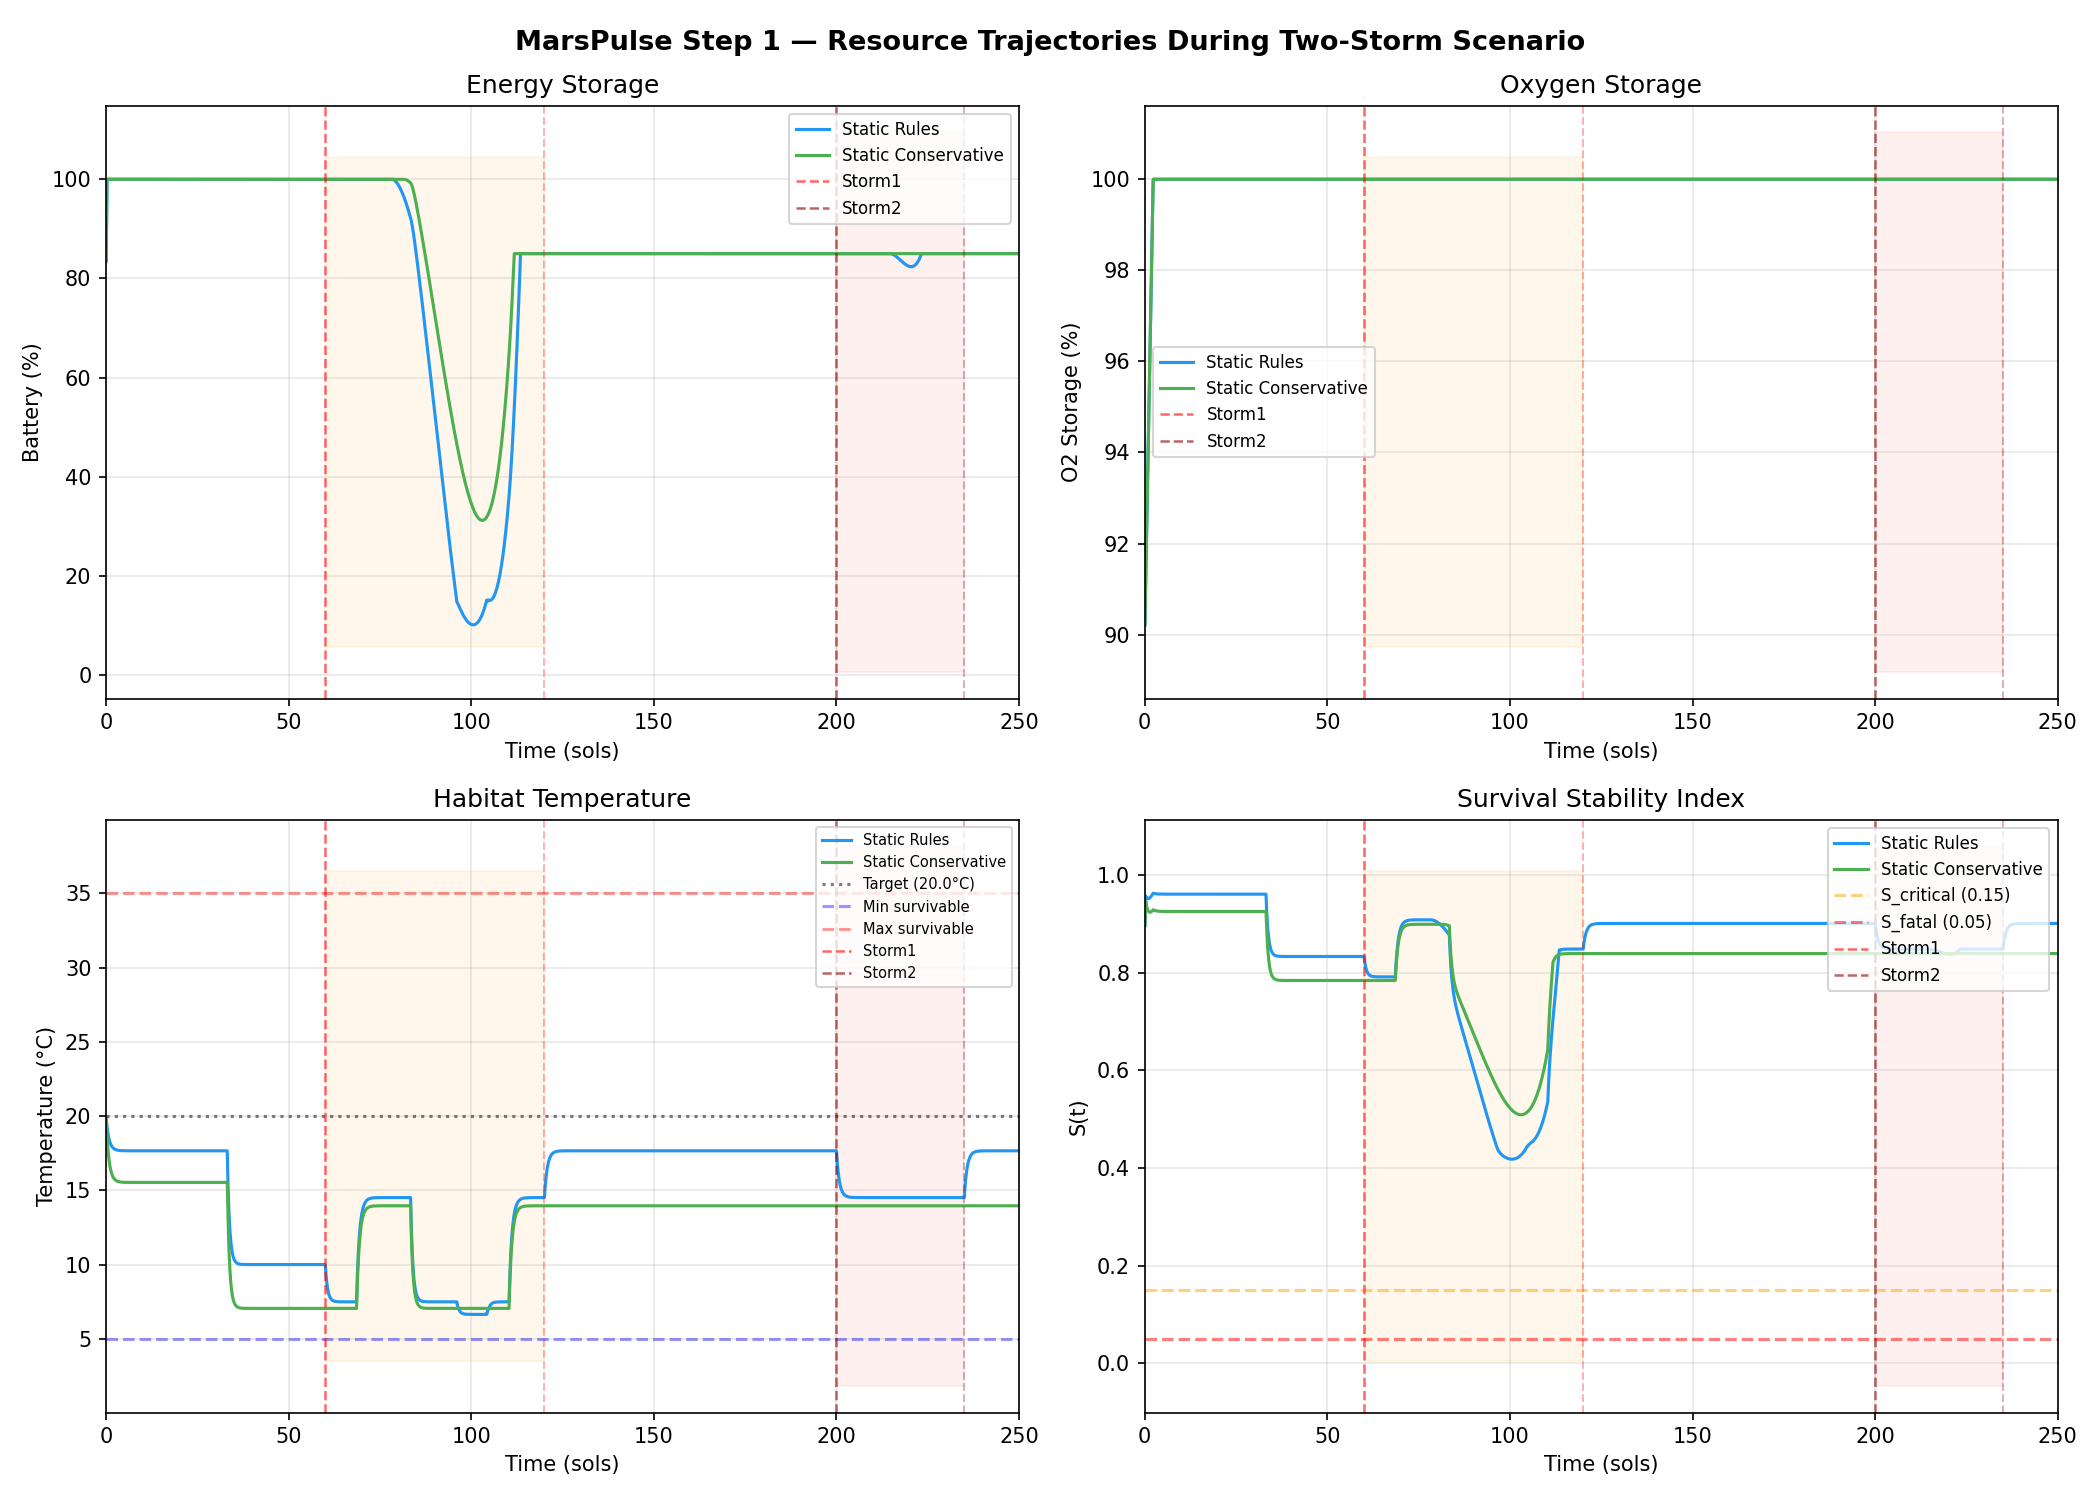
\includegraphics[width=0.85\textwidth]{step1_trajectories.png}
  \caption{Resource trajectories for static rule agents (representative episode with full 300-sol survival). The first storm (sol~60--120, orange shading) drives progressive battery decline; Storm~2 (sol~200--235, red shading) shows a second dip in available power. Temperature declines gradually through both storms toward the lower survivable bound. Both trajectory curves are visible across the full 0--250~sol time axis.}
  \label{fig:traj}
\end{figure}

\subsection{Step 2: MAPPO Training}

Training progressed from approximately 1.5~sols (random initialization) to 135+~sols (surviving through Storm~1) over 300,000 steps. Figure~\ref{fig:training} shows two key indicators: reward rises steadily with training (trend $r = +0.775$, $p < 0.001$), and critic loss converges consistently, indicating the centralized critic learns reliable global value estimates.

\begin{figure}[H]
  \centering
  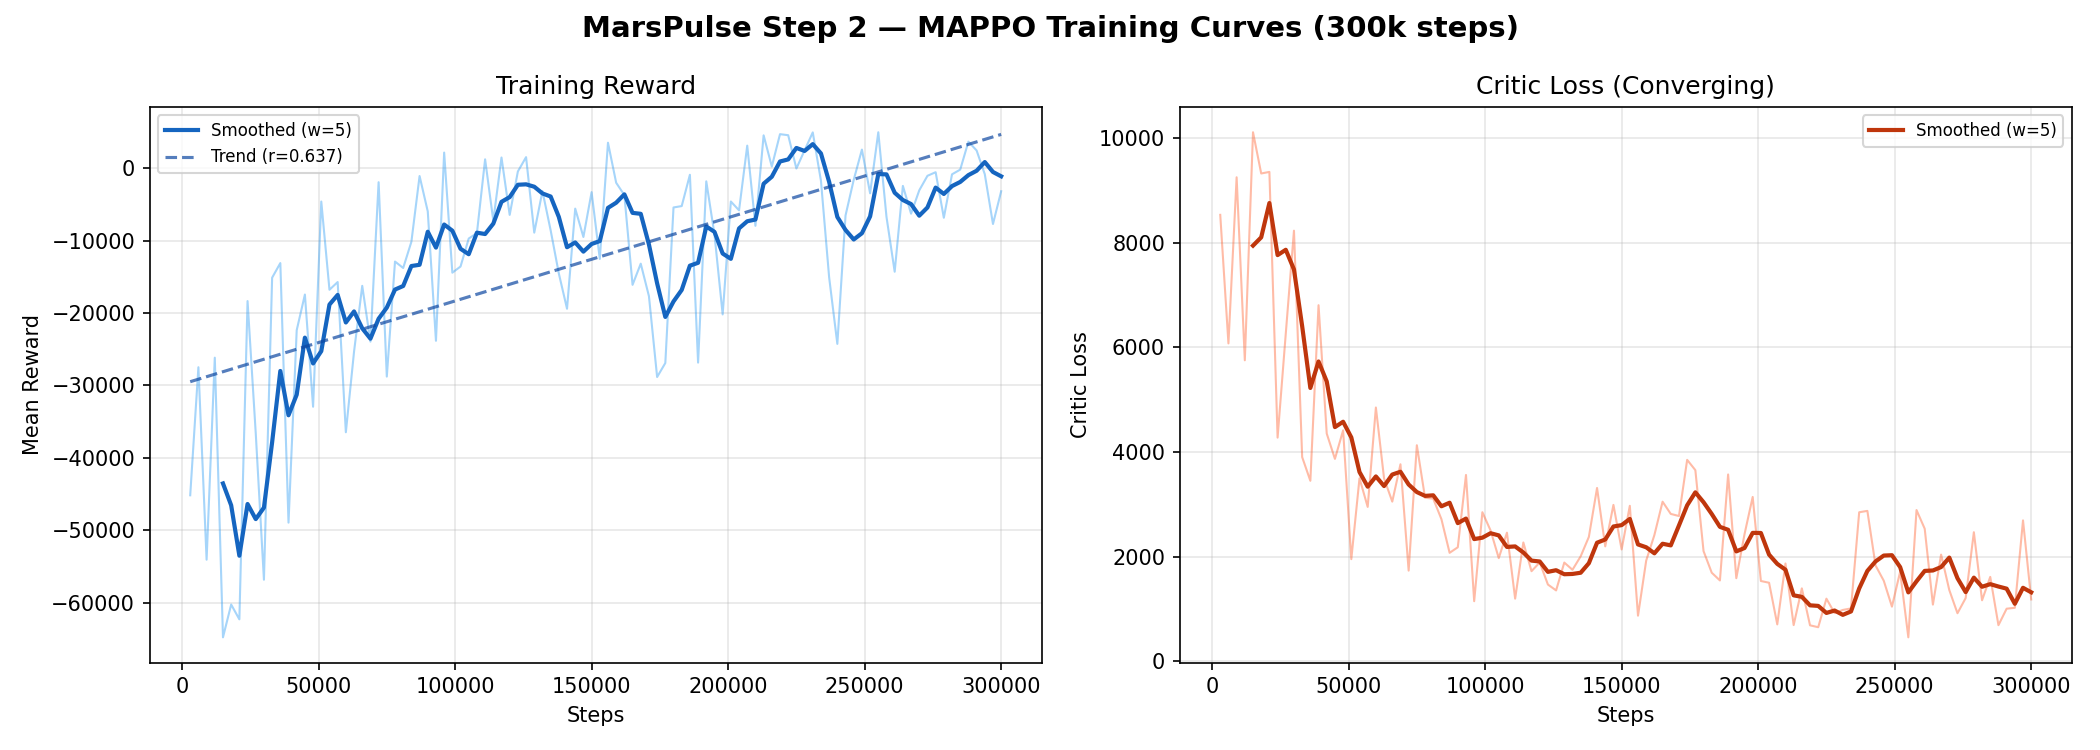
\includegraphics[width=0.85\textwidth]{step2_training.png}
  \caption{Training curves. Left: mean episode reward per epoch (light blue raw, dark blue moving average, dashed linear trend with $r = +0.775$). Right: critic loss converging steadily.}
  \label{fig:training}
\end{figure}

\begin{table}[H]
  \centering
  \caption{Step 2: MARL vs.\ static baseline (100 episodes)}
  \label{tab:step2}
  \begin{tabular}{@{}lcccc@{}}
    \toprule
    \textbf{Agent} & \textbf{Survival (sols)} & \textbf{Fatality} & \textbf{Full 300-sol} & \textbf{Mean S} \\
    \midrule
    Static Rules & $123.7 \pm 75.6$ & 92\% & 8\% & 0.862 \\
    Static Conservative & $111.0 \pm 70.0$ & 96\% & 4\% & 0.840 \\
    MAPPO MARL & $\mathbf{167.2 \pm 116.7}$ & \textbf{63\%} & \textbf{37\%} & 0.756 \\
    \bottomrule
  \end{tabular}
\end{table}

MAPPO extends mean survival from the best static baseline's 123.7~sols to 167.2~sols (+35.2\%) and achieves a substantially higher full-survival rate (37\% vs.\ 8\% for static). The improvement comes with increased variance ($\sigma = 116.7$ vs.\ 75.6~sols). The distribution is bimodal: episodes either survive both storms ($\sim$300~sols) or fail very early ($\sim$2~sols, roughly 20\% of runs), with the remainder distributed through the storm periods. The early-failure tail corresponds to episodes where a poor initial action sequence triggers cascading resource failure before the policy stabilizes.

\begin{figure}[H]
  \centering
  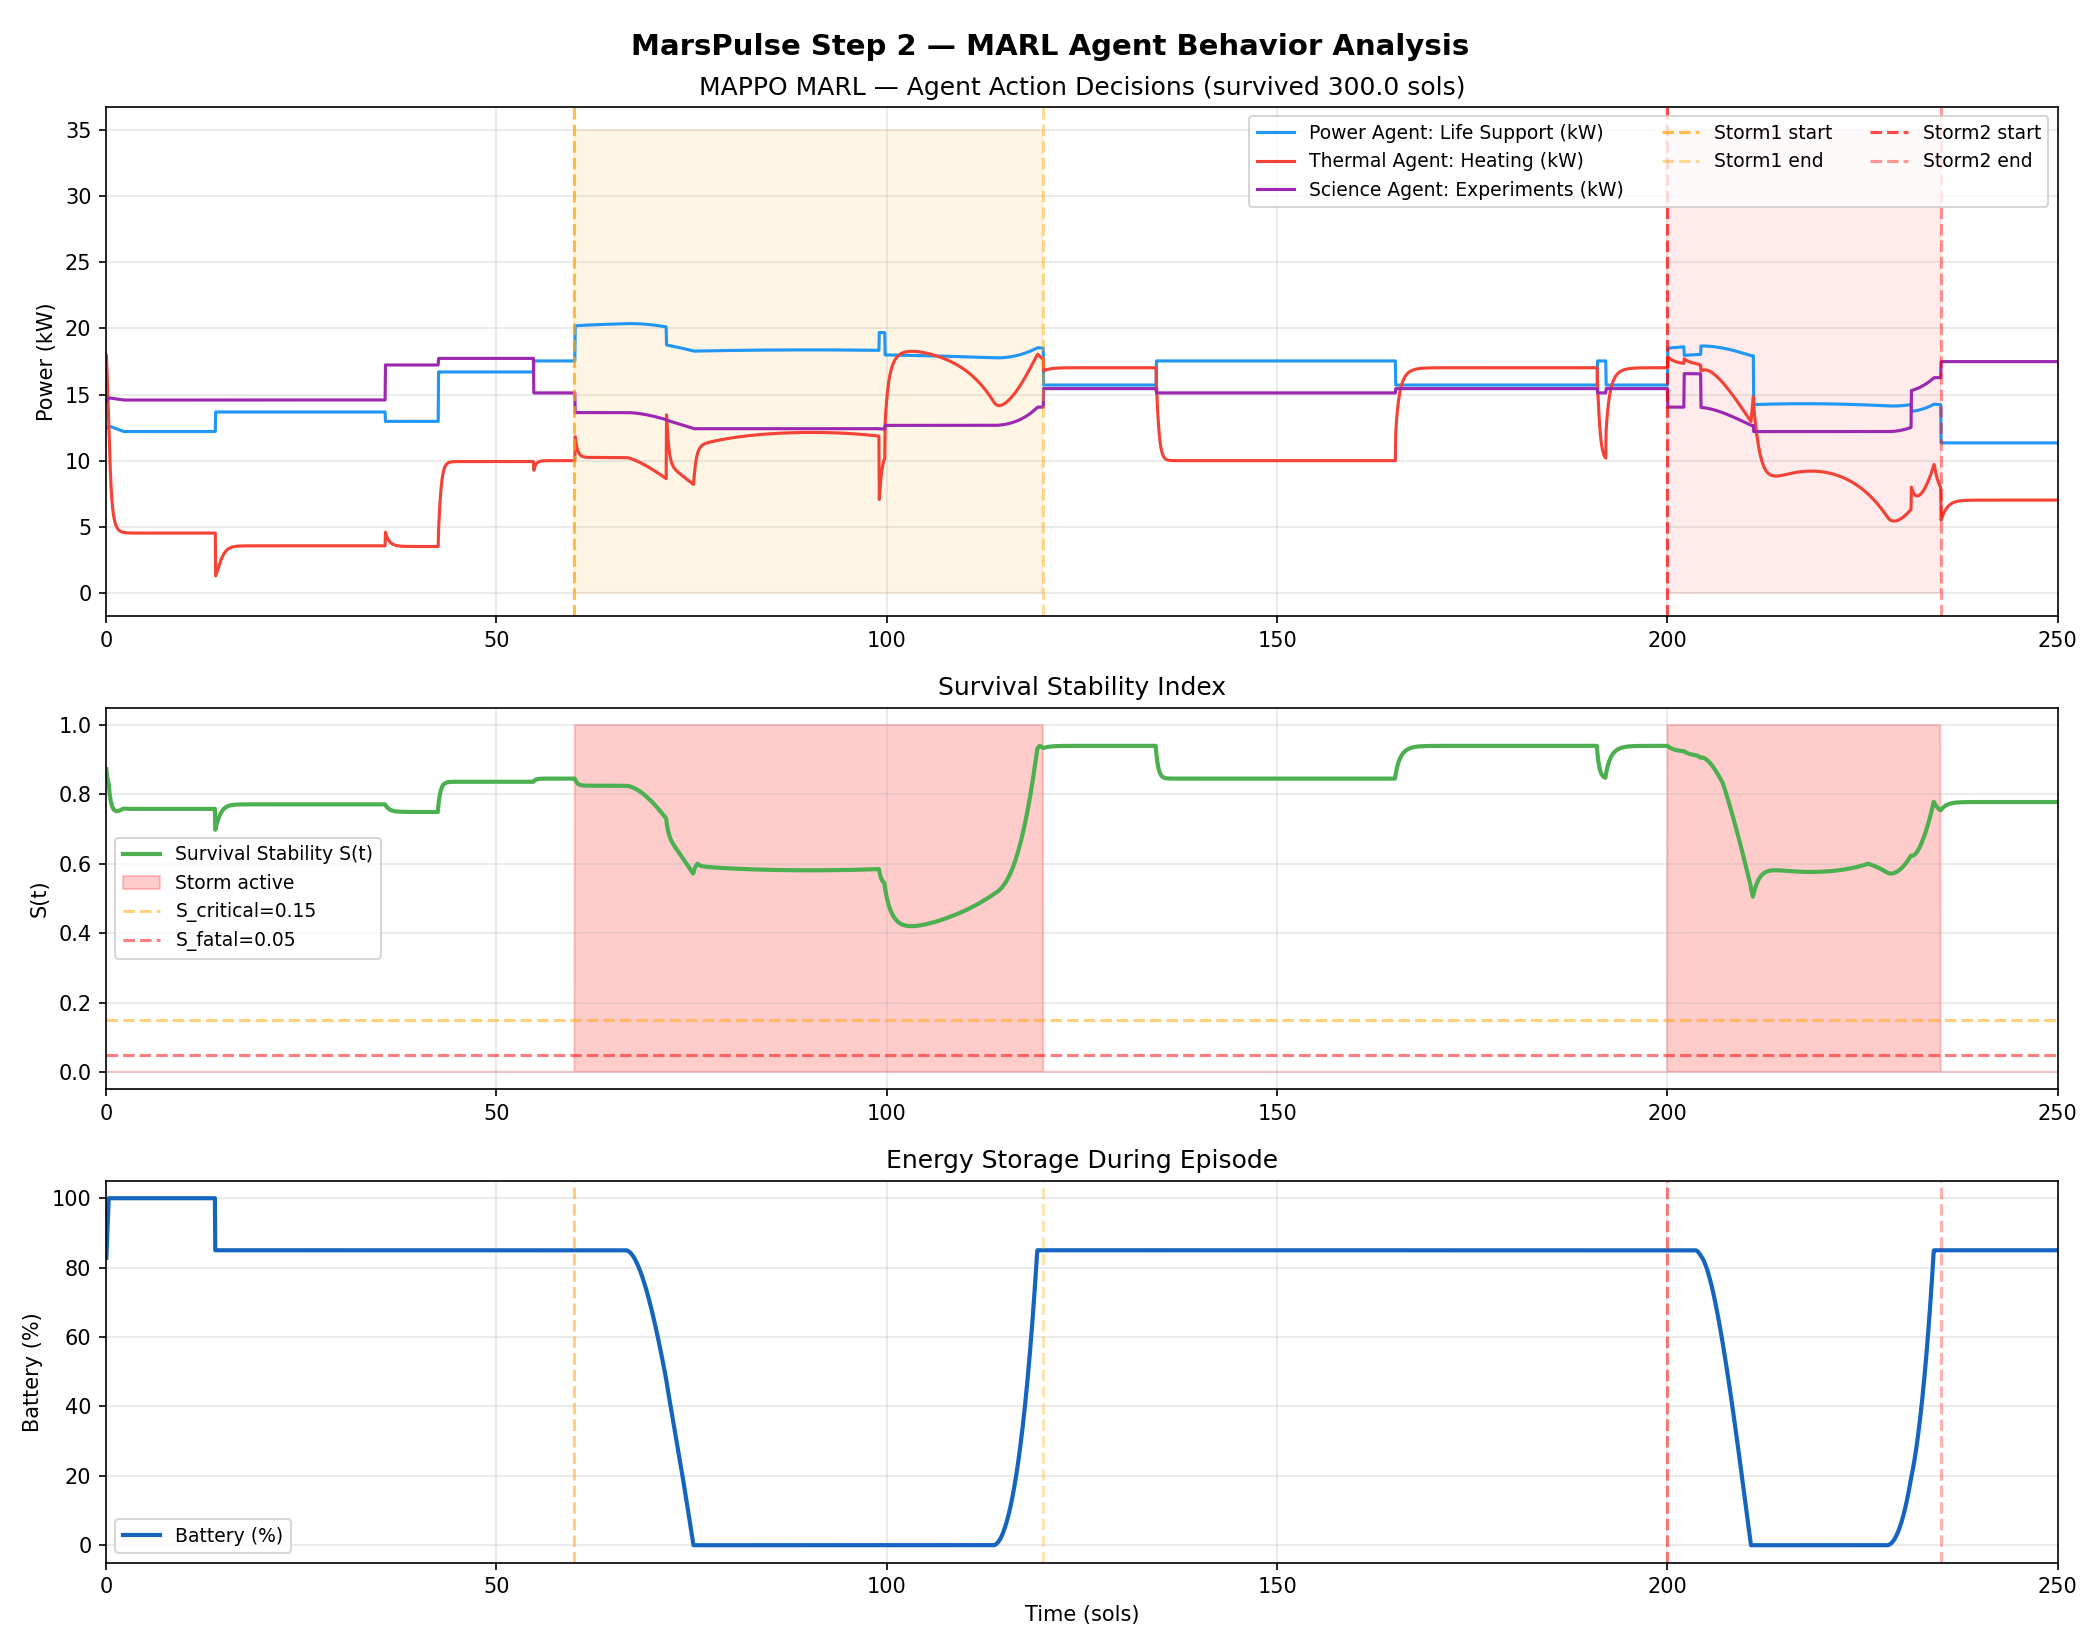
\includegraphics[width=0.85\textwidth]{step2_agent_actions.png}
  \caption{Agent power allocations during a representative episode with full 300-sol survival. Top: the Science Agent (purple) shuts down experiments during both storms (orange and red shaded regions). The Thermal Agent (red) maintains heating with modest reductions during storms, exploiting the lava tube's thermal inertia. The Power Agent (blue) holds life support near nominal levels. Middle: evolution of the Survival Stability Index $S(t)$. Bottom: battery state-of-charge across the full episode.}
  \label{fig:actions}
\end{figure}

\subsection{Step 3: Sensitivity \& Failure Analysis}

\subsubsection{Parameter Sweeps}

We swept storm optical depth $\tau$, battery capacity, and RTG power while evaluating the static rules agent (20 episodes per point).

\begin{figure}[H]
  \centering
  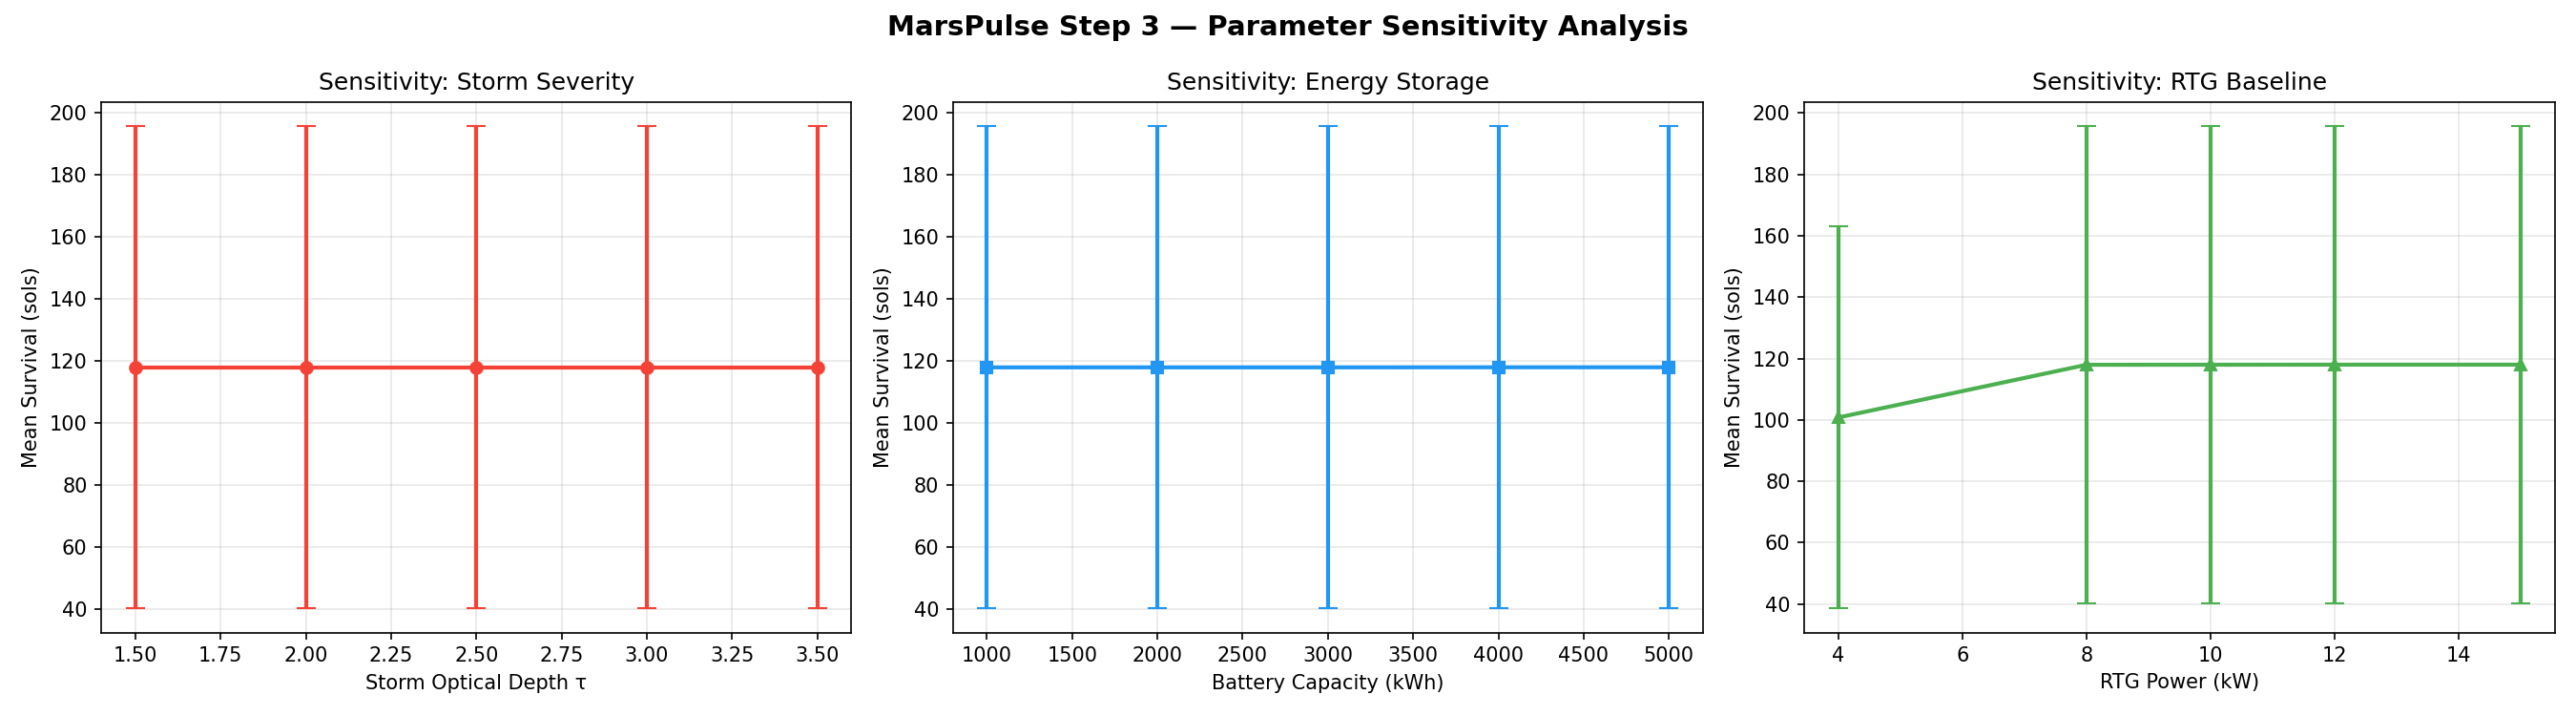
\includegraphics[width=0.95\textwidth]{step3_sensitivity.png}
  \caption{Parameter sensitivity for the static agent. Left: storm $\tau$. Center: battery capacity. Right: RTG baseline power. Error bars $\pm 1\sigma$.}
  \label{fig:sensitivity}
\end{figure}

The most striking result is the flatness of the response. Static agent survival holds at $\sim$118~sols for $\tau = 1.5$ through $\tau = 3.0$, and at $\sim$118~sols for battery capacities from 1,000 through 5,000~kWh. Only the most extreme parameter values move the needle: $\tau = 3.5$ drops survival to $\sim$100~sols, and RTG power below 8~kW reduces it to $\sim$101~sols. A fivefold increase in battery capacity provides no survival benefit because the agent's curtailment logic wastes the extra stored energy before the storm.

This is a \textit{decision ceiling}, not a physics ceiling. The static agent fails at approximately the same point regardless of hardware because its fixed-threshold rules do not permit the pre-storm conservation that would let a larger battery or milder storm matter. This is the limitation that learned anticipatory behavior is intended to address.

\subsubsection{Failure Mode Impact}

\begin{table}[H]
  \centering
  \caption{Failure mode impact (20 episodes each, static agent)}
  \label{tab:failures}
  \begin{tabular}{@{}lc@{}}
    \toprule
    \textbf{Condition} & \textbf{Survival (sols)} \\
    \midrule
    No failure (baseline) & $118.0 \pm 77.7$ \\
    \midrule
    \textit{Single failure:} & \\
    \quad Electrolysis degraded & $83.3 \pm 33.8$ \\
    \quad Heater fault & $81.8 \pm 52.2$ \\
    \quad Battery cell failure & $115.9 \pm 80.0$ \\
    \quad Habitat leak & $83.2 \pm 44.5$ \\
    \midrule
    \textit{Compound failures:} & \\
    \quad Heater fault + Habitat leak & $\mathbf{74.2 \pm 52.3}$ \\
    \quad Heater fault + Battery failure & $100.0 \pm 63.6$ \\
    \quad Electrolysis + Habitat leak & $85.6 \pm 34.2$ \\
    \bottomrule
  \end{tabular}
\end{table}

Heater fault and habitat leak individually reduce survival by roughly 35~sols each; together they produce the worst outcome at 74.2~sols. This is a thermal collapse mode: the habitat loses heat faster than the degraded heater can replenish it. Battery cell failure, counterintuitively, slightly \textit{increases} mean survival (115.9 vs.\ 118.0~sols) because the reduced effective capacity triggers more conservative load shedding earlier in the episode---an accidental benefit of a rule architecture designed for a different failure mode.

\subsubsection{Survival Surface}

\begin{figure}[H]
  \centering
  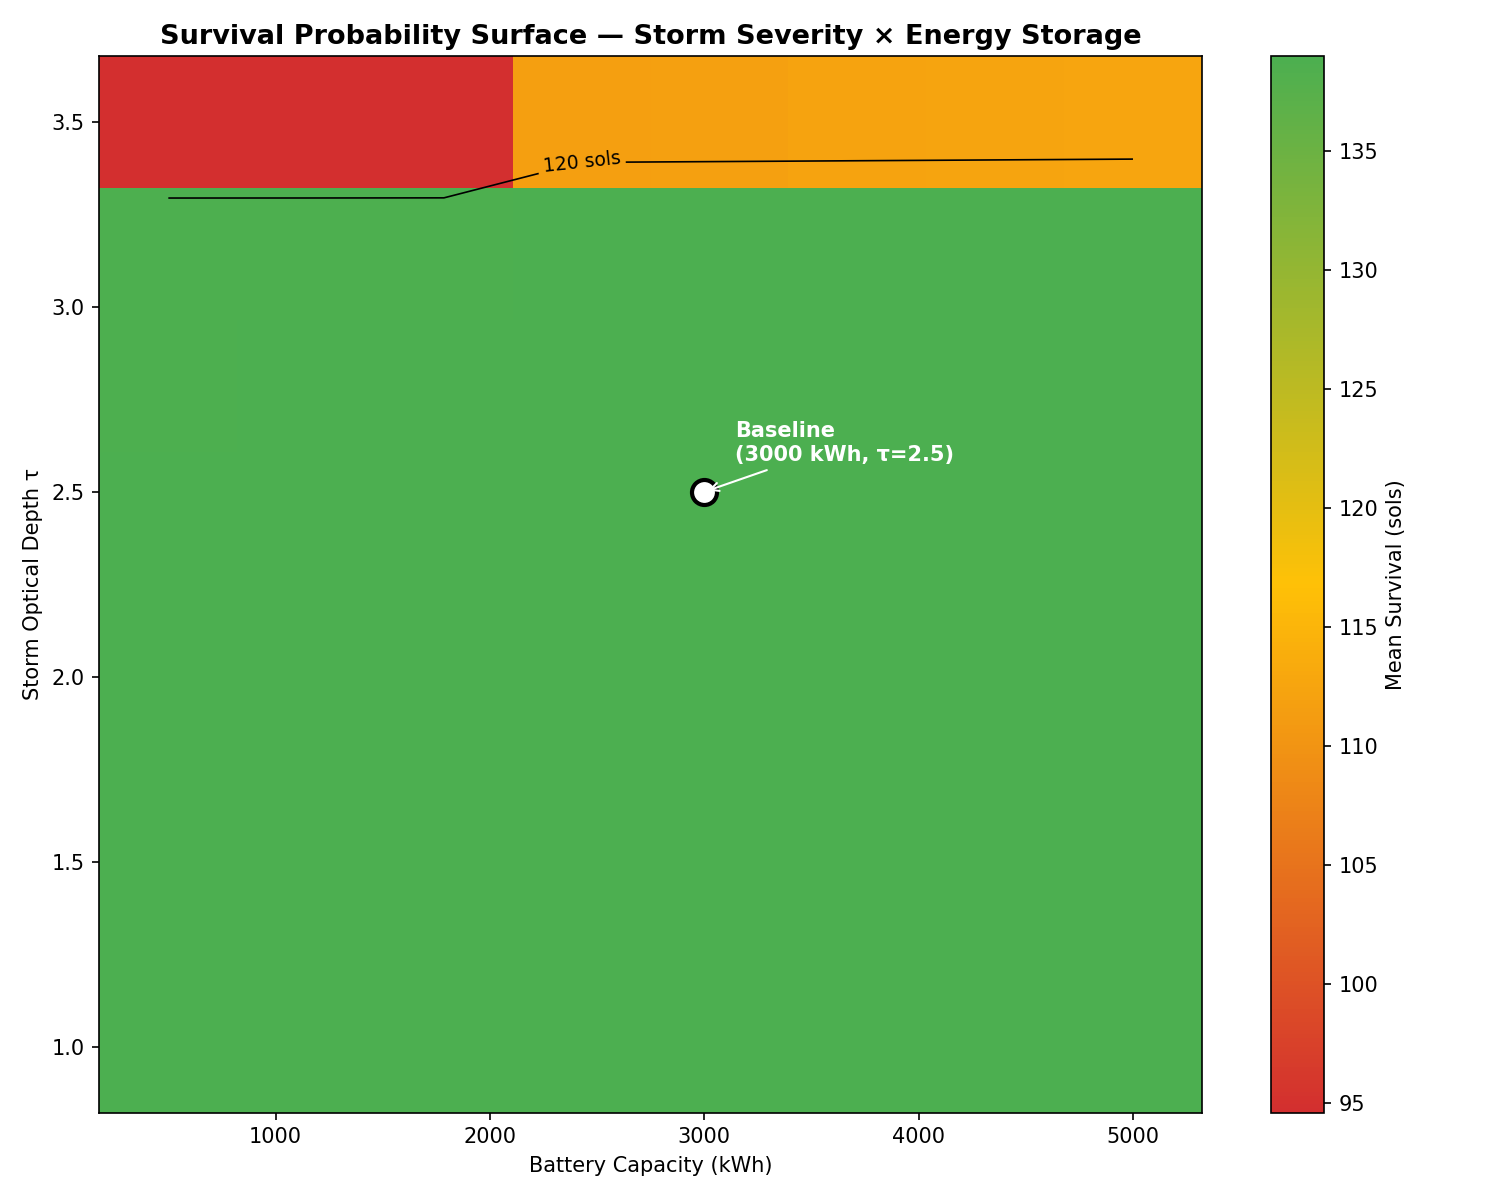
\includegraphics[width=0.75\textwidth]{step3_survival_surface.png}
  \caption{Survival surface over $\tau$ and battery capacity for the static agent. Contours show iso-survival levels. The white star marks the baseline configuration (3,000~kWh, $\tau = 2.5$).}
  \label{fig:surface}
\end{figure}

\subsection{Step 4: Ablation --- What Does the Central Critic Buy?}

To isolate the effect of the centralized critic, we compared four configurations:

\begin{table}[H]
  \centering
  \caption{Ablation results (50 episodes each). \textbf{Note:} MAPPO fatality is 70\% here vs.\ 62\% in Step~2 because the ablation experiment uses different training configurations and evaluation seed sets. Both values are compared against baselines within their respective experiments.}
  \label{tab:ablation}
  \begin{tabular}{@{}lccc@{}}
    \toprule
    \textbf{Method} & \textbf{Survival (sols)} & \textbf{Fatality} & \textbf{$\Delta$ vs.\ Static} \\
    \midrule
    Static Rules & $114.1 \pm 73.8$ & 92\% & --- \\
    Single-Agent PPO & $2.5 \pm 0.2$ & 100\% & $-$111.6 \\
    Independent PPO $\times$3 & $2.4 \pm 0.2$ & 100\% & $-$111.7 \\
    MAPPO (central critic) & $\mathbf{129.7 \pm 122.2}$ & 70\% & +15.6 \\
    \bottomrule
  \end{tabular}
\end{table}

\begin{figure}[H]
  \centering
  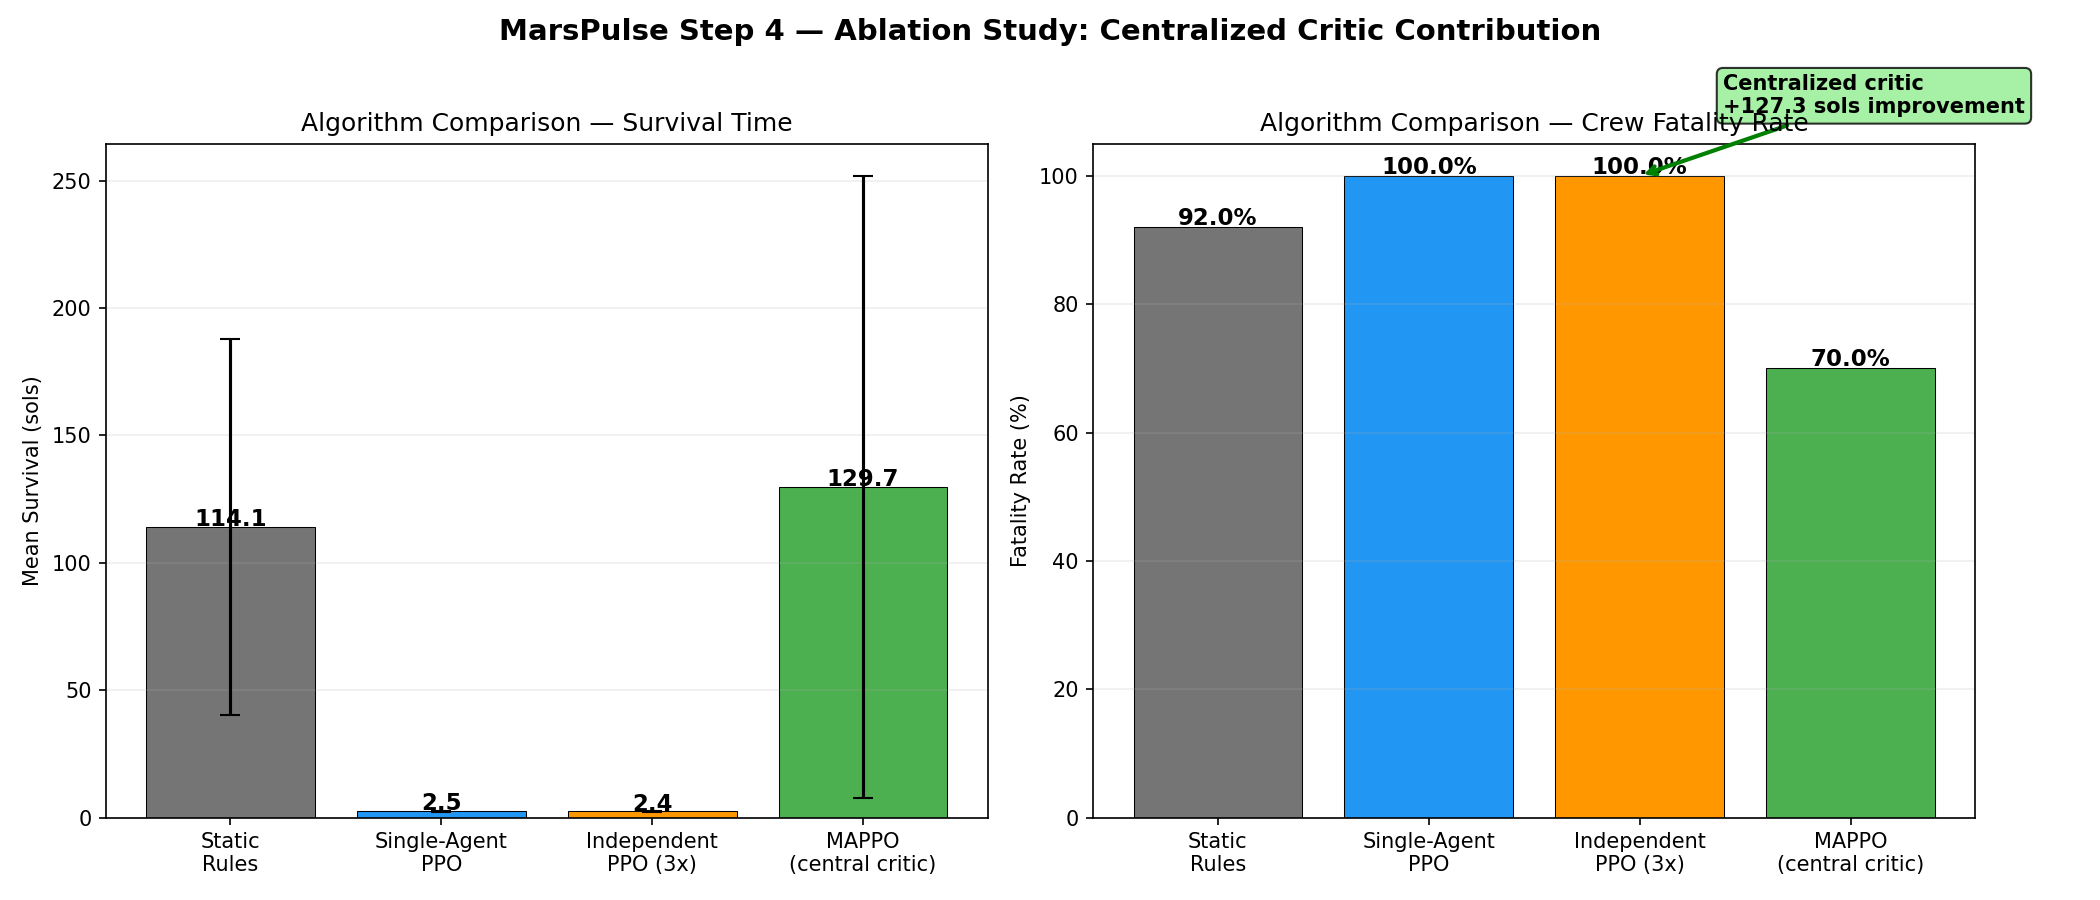
\includegraphics[width=0.9\textwidth]{step4_ablation.png}
  \caption{Ablation results. Left: mean survival. Right: fatality rates. The centralized critic provides a 127.3-sol improvement over independent PPO.}
  \label{fig:ablation}
\end{figure}

The single-agent and independent PPO results are not a typo: both collapse to roughly 2.5~sols, dying almost immediately. The 300-sol, two-storm scenario creates a credit assignment problem severe enough that monolithic or uncoordinated RL cannot learn even the most basic survival behavior. The centralized critic bridges this gap, providing a 127.3-sol improvement (2.4 $\rightarrow$ 129.7~sols, roughly 54$\times$). Three factors explain the gap:

\begin{enumerate}[label=(\arabic*)]
  \item \textbf{Multi-objective interference in the single-agent case:} A monolithic policy must simultaneously manage energy, oxygen, and thermal objectives whose gradients can oppose each other. The resulting compromise satisfies none of the constraints well.
  \item \textbf{Resource contention without coordination:} Three independent agents each try to maximize the shared reward by consuming from the common battery. Within a few timesteps they collectively drain reserves because no agent's local value function represents the effect of its actions on the others' future resource availability.
  \item \textbf{Global state visibility:} The centralized critic $V_\phi(s, \mathbf{a})$ sees the full state and joint action, enabling it to learn that, e.g., the power agent's life support allocation provides waste heat that the thermal agent can use, or that high experiment loads during clear-sky periods leave the battery unprepared for storms.
\end{enumerate}

%======================================================================
\section{Discussion}
%======================================================================

\subsection{What the Learned Policy Does Differently}

Comparing the MAPPO agent action traces (Figure~\ref{fig:actions}) with static rule traces (Figure~\ref{fig:traj}) reveals specific behavioral differences:

\begin{enumerate}[label=(\arabic*)]
  \item \textbf{Pre-storm preparation:} The static agent maintains full experimental power (18~kW) right up to the moment an energy threshold is breached, typically 10--15~sols into the storm. The MARL policy begins reducing experiments as soon as the storm onset is detected (via the optical depth observation), sometimes even earlier when the storm-status flag activates. This preserves 15--20~sols' worth of battery charge that the static agent wastes.

  \item \textbf{Context-dependent curtailment:} Static rules enforce a rigid hierarchy. MARL agents adjust based on multiple signals simultaneously: when O$_2$ is abundant and temperature is stable, the power agent can briefly reduce life support to preserve battery; when temperature approaches the lower bound, the thermal agent requests more heating and the science agent yields.

  \item \textbf{Cross-subsystem coupling:} Because the central critic models joint effects, the thermal agent learns to ``coast'' on waste heat from life support equipment (roughly 70\% of electrical power is dissipated as heat), reducing its own heating demand during periods of high life support activity.
\end{enumerate}

\subsection{The Bimodal Outcome Distribution}

The high variance of the MAPPO policy ($\sigma = 116.7$~sols) is not a training failure but a signature of the policy operating near a critical threshold. In roughly 20\% of evaluation episodes, the policy outputs an action sequence in the first few timesteps that triggers a cascade---battery drains, O$_2$ generation stops, temperature drops---before the policy can stabilize. In the remaining 80\%, it survives through the first storm, and in 38\% it survives both storms.

This bimodality is common in learned policies for environments with sharp failure boundaries: small differences in the initial action sequence can produce qualitatively different trajectories. It also points to a direction for future improvement: techniques that constrain early-episode exploration (safe RL, shielding, or behavioral cloning from successful trajectories) could eliminate the early-failure mode and potentially raise the full-survival rate above 50\%.

\subsection{When Coordination Becomes Necessary}

The ablation results suggest that the value of the centralized critic scales with task complexity. In the original 60-sol, single-storm benchmark (from earlier project phases), independent PPO achieved $\sim$44.5~sols vs.\ $\sim$46.3~sols for static rules---a small gap. In the 300-sol, two-storm scenario, independent PPO achieves 2.4~sols vs.\ 114.1~sols for static rules. The difference is not just quantitative but qualitative: at a certain horizon length, uncoordinated multi-agent learning ceases to work at all.

This has practical implications for engineering autonomous space systems. If the expected autonomy horizon is short (hours to days), simple rule-based controllers or lightly-coordinated RL may be adequate. For multi-month blackout scenarios, architectural coordination mechanisms become essential. The crossover point and its dependence on scenario parameters (number of agents, storm severity, resource margins) warrant further study.

%======================================================================
\section{Conclusion}
%======================================================================

This project developed and evaluated a MAPPO-based resource management system for a simulated Mars lava tube base under a challenging two-storm, 300-sol scenario. The main findings are:

\begin{enumerate}[label=(\arabic*)]
  \item A three-agent decomposition (power, thermal, science) with a centralized critic learns to coordinate resource allocation in ways that static rule-based controllers cannot match. In a same-seed 100-episode evaluation, mean survival improves from 123.7 to 167.2~sols (+35.2\%), and the full-survival rate goes from 8\% to 37\%.
  \item The centralized critic is load-bearing, not cosmetic. Removing it (independent PPO) causes the policy to collapse to $\sim$2.5~sols, performing far worse than even the static baseline. The critic contributes +127.3~sols over the uncoordinated case.
  \item Static agent survival is dominated by decision architecture rather than hardware parameters. A fivefold increase in battery capacity produces no change in survival time under static rules ($\sim$118~sols for all values), because fixed-threshold logic cannot perform the anticipatory conservation needed to exploit additional storage.
  \item The most dangerous compound failure mode is heater fault combined with habitat leak (74.2~sols mean survival under static rules), reinforcing the importance of thermal system redundancy in subsurface base design.
\end{enumerate}

Several directions remain open. The bimodal outcome distribution (early failures vs.\ full survival) suggests safe exploration techniques could substantially improve worst-case performance. The current thermal model uses lumped parameters; spatially resolved modeling would better capture the lava tube geometry's effect on heat flow. Extending the scenario to multi-year durations with seasonal storm cycles would test whether the policy can learn resource management across longer timescales with periodic replenishment opportunities.

On the engineering deployment side, two extensions have been completed: (1)~an interactive HTML5 visualization dashboard (\texttt{report\_dashboard.html}) that renders the six-panel analysis and performance matrix in a web browser; and (2)~a policy export tool (\texttt{export\_unihiker\_policy.py}) that converts the trained MAPPO model weights to NumPy format for deployment on the UniHiker embedded platform, driving WS2812B LED strips and an SSD1306 OLED display to demonstrate Mars base resource management as a physical interactive exhibit.

\vspace{20pt}
\begin{flushright}
  --- MarsPulse Research Team
\end{flushright}

%======================================================================
\section*{Acknowledgments}
This project was developed for the deep space exploration and aerospace + AI research themes. The MAPPO implementation builds on open-source tools from the reinforcement learning community, including Gymnasium~\cite{gymnasium} and PyTorch~\cite{pytorch}.

%======================================================================
\begin{thebibliography}{99}

\bibitem{mappo}
C.~Yu, A.~Velu, E.~Vinitsky, J.~Gao, Y.~Wang, A.~Bayen, and Y.~Wu,
``The Surprising Effectiveness of PPO in Cooperative Multi-Agent Games,''
in \textit{Advances in Neural Information Processing Systems (NeurIPS)}, vol.~35, pp.~24611--24624, 2022.

\bibitem{ppo}
J.~Schulman, F.~Wolski, P.~Dhariwal, A.~Radford, and O.~Klimov,
``Proximal Policy Optimization Algorithms,''
\textit{arXiv preprint arXiv:1707.06347}, 2017.

\bibitem{gae}
J.~Schulman, P.~Moritz, S.~Levine, M.~I. Jordan, and P.~Abbeel,
``High-Dimensional Continuous Control Using Generalized Advantage Estimation,''
in \textit{Proc. International Conference on Learning Representations (ICLR)}, 2016.

\bibitem{maddpg}
R.~Lowe, Y.~Wu, A.~Tamar, J.~Harb, P.~Abbeel, and I.~Mordatch,
``Multi-Agent Actor-Critic for Mixed Cooperative-Competitive Environments,''
in \textit{Advances in Neural Information Processing Systems (NeurIPS)}, pp.~6379--6390, 2017.

\bibitem{qmix}
T.~Rashid, M.~Samvelyan, C.~S. de~Witt, G.~Farquhar, J.~N. Foerster, and S.~Whiteson,
``QMIX: Monotonic Value Function Factorisation for Deep Multi-Agent Reinforcement Learning,''
in \textit{Proc. International Conference on Machine Learning (ICML)}, pp.~4295--4304, 2018.

\bibitem{mars_lava_tube}
P.~J. Boston, D.~E. Northup, and M.~N. Spilde,
``Cave Biosignature Suites: Microbes, Minerals, and Mars,''
\textit{Astrobiology}, vol.~1, no.~1, pp.~25--55, 2001.

\bibitem{mars_dust}
M.~D. Smith,
``Spacecraft Observations of the Martian Atmosphere,''
\textit{Annual Review of Earth and Planetary Sciences}, vol.~36, pp.~191--219, 2008.

\bibitem{mars_isru}
D.~Rapp,
\textit{Use of Extraterrestrial Resources for Human Space Missions to Moon or Mars},
2nd ed., Springer, 2018.

\bibitem{nasa_ls}
NASA,
``Life Support Baseline Values and Assumptions Document,''
NASA/TP-2015-218570, 2015.

\bibitem{mars_radiation}
D.~M. Hassler \textit{et al.},
``Mars' Surface Radiation Environment Measured with the Mars Science Laboratory's Curiosity Rover,''
\textit{Science}, vol.~343, no.~6169, 1244797, 2014.

\bibitem{kilopower}
M.~A. Gibson \textit{et al.},
``Kilopower: NASA's Small Fission Power System for Science and Human Exploration,''
in \textit{Proc. Nuclear and Emerging Technologies for Space (NETS)}, 2018.

\bibitem{gymnasium}
M.~Towers \textit{et al.},
``Gymnasium: A Standard Interface for Reinforcement Learning Environments,''
\textit{arXiv preprint arXiv:2407.17032}, 2024.

\bibitem{pytorch}
A.~Paszke \textit{et al.},
``PyTorch: An Imperative Style, High-Performance Deep Learning Library,''
in \textit{Advances in Neural Information Processing Systems (NeurIPS)}, pp.~8024--8035, 2019.

\bibitem{mars_thermal}
R.~D. Braun and R.~M. Manning,
``Mars Exploration Entry, Descent, and Landing Challenges,''
\textit{Journal of Spacecraft and Rockets}, vol.~44, no.~2, pp.~310--323, 2007.

\bibitem{marl_survey}
P.~Hernandez-Leal, B.~Kartal, and M.~E. Taylor,
``A Survey and Critique of Multiagent Deep Reinforcement Learning,''
\textit{Autonomous Agents and Multi-Agent Systems}, vol.~33, no.~6, pp.~750--797, 2019.

\end{thebibliography}

\end{document}
